
\فصل{کارهای پیشین}
\قسمت{الگوریتم‌های کوانتومی در هندسهٔ محاسباتی}

استفاده از ابزارِ رایانشِ کوانتومی در هندسهٔ محاسباتی از بدوِ پیدایشِ این شاخه و توسعهٔ الگوریتم‌های مشهورِ آن، موردِ بررسی قرار گرفته \مرجع{sadakane} اما با این‌حال تا امروزه ادبیاتِ کاملاً محدودی وجود دارد که الگوریتم‌ها و حدهایی در آن به صورتِ‌ موردی بررسی شده‌اند. هرچند تعدادِ این حدود و الگوریتم‌ها کم نیست اما هنوز تلاش‌ها در جهتِ تعمیم و کلیت‌بخشی به این گزاره‌ها چندان زیاد نبوده‌اند.

همچنین نکتهٔ مهمی که حائزِ اهمیتِ بیشتری‌ست این است که بیشترِ تلاش‌ها در این حوزه معطوف به استفاده از الگوریتم‌های جست‌وجو، شمارش و یا ولگشت‌های کوانتومی هستند که بهبودِ سرعتِ آن‌ها در نهایت می‌تواند به شکلِ مربعی \زیرنویس{\lr{quadratic}} باشد. و به نظر می‌رسد هنوز از الگوریتم‌هایی که بهبودِ سرعتِ توانی
\زیرنویس{\lr{exponential}} دارند در این حوزه استفاده‌ای نشده‌است. \مرجع{bahadur}\مرجع{volpato}\مرجع{lanzagorta}\مرجع{ambainis}\مرجع{buhrman}

در ادامه به بررسیِ الگوریتم‌ها و حدود در تلاش‌های پیشین می‌پردازیم.

از آن‌جا که هدف از این بررسی‌ها، بستگیِ پیچیدگیِ محاسباتی به پارامترهایی نظیرِ بعد و دقتِ ارقام نیست، در مرتبهٔ الگوریتم‌ها و حدها ثابت فرض شده‌اند و نوشته‌نشده‌اند.

\متن‌سیاه{مسئلهٔ برخوردِ اجسامِ محدب}: در فضای $d$-بعدی در نظر بگیرید که $N$ شکلِ محدب داریم، هدف فهمیدنِ این است که آیا وجود دارد دوتایی از این اجسام که با هم تلاقی داشته‌باشند. \مرجع{sadakane}
\شروع{شمارش}[-]
\فقره {الگوریتمِ کلاسیک}:
\فقره {حدِ کلاسیک}:
\فقره {الگوریتمِ کوانتومی}:
\فقره {حد کوانتومی}:
\پایان{شمارش}

\متن‌سیاه{مسئلهٔ پوش محدب}
% Convex hull computation

\متن‌سیاه{مسئلهٔ چیدمانِ ابرصفحه‌ها\زیرنویس{\lr{arrangement of hyperplanes}}}
% Let A be an arrangement of nphyperplanes
% in the d-dimensional space.

\متن‌سیاه{مسئلهٔ محاسبهٔ فاصلهٔ هاسدورف}
% Hausdorff distance computation


\متن‌سیاه{مسئلهٔ نزدیک‌ترین زوج}: 
\(N\)
نقطه در فضای \(d\)-بعدی و یک تابعِ فاصله 
\(d: \mathbb{R}^d \times \mathbb{R}^d \to \mathbb{R}^+\)
داده‌شده‌اند، مطلوب است زوجی که کم‌ترین فاصله را دارند. \مرجع[فصل پنجم]{preparata}\مرجع{volpato}

\شروع{شمارش}[-]
\فقره {الگوریتمِ کلاسیک}: با استفاده از تقسیم و حل، با 
$\Theta(N \log N)$ 
مقایسه (بینِ فاصلهٔ زوج‌نقاط)
امکانِ حل وجود دارد.
البته برای الگوریتم‌های تصادفی، الگوریتم با امیدریاضیِ تعدادِ مقایسه‌ها
$\Theta(N)$
ممکن است.
\فقره {حدِ کلاسیک}: با استفاده از یکتاییِ عناصر، مقایسه‌ها باید از مرتبهٔ
$\Omega(N \log N)$
باشند.

\فقره {الگوریتمِ کوانتومی}: با استفاده از کاهش (با سربارِ لگاریتمی) به الگوریتمِ پیدا کردنِ کمینهٔ کوانتومی، با
$\Theta(N^{\frac{2}{3}} \log N)$
پرسشِ مقایسه، مسئله حل می‌شود.
\فقره {حد کوانتومی}: با استفاده از یکتاییِ عناصر به شکلِ کوانتومی به حدِ
$\O{N^{\frac{2}{3}}}$
خواهیم رسید.

\پایان{شمارش}

\متن‌سیاه{مسئلهٔ دورترین زوج}: 
\(N\)
نقطه در فضای \(d\)-بعدی و یک تابعِ فاصله 
\(d: \mathbb{R}^d \times \mathbb{R}^d \to \mathbb{R}^+\)
داده‌شده‌اند، مطلوب است زوجی که بیشترین فاصله را دارند.
 
نتایجِ آن مشابهِ مسئلهٔ نزدیک‌ترین زوج هستند.\مرجع{volpato}

\متن‌سیاه{مسئلهٔ نزدیک‌ترین زوجِ دورنگ}: 
$N$
نقطهٔ آبی و $M$ نقطهٔ قرمز و یک تابعِ فاصله 
\(d: \mathbb{R}^d \times \mathbb{R}^d \to \mathbb{R}^+\)
داده‌شده‌اند، مطلوب است زوجِ ناهم‌رنگی که کم‌ترین فاصله را دارند. \مرجع{volpato}\cite[\lr{Minimum Geometric Spanning Trees}]{kao}

\شروع{شمارش}[-]
\فقره {الگوریتمِ کلاسیک}: با استفاده از زیردرختِ پوششیِ کمینهٔ هندسی، برای فاصله‌های خاصی نظیرِ $L_1$ در زمانِ 
$\O{(N+M) \log (N+M)}$
 امکانِ حل وجود دارد.

با استفاده از الگوریتم‌های تصادفی نیز در زمانِ
$\O{(NM \log N\log M)^\frac{2}{3}+N\log^2M+M\log^2N}$
حل می‌شود.
\فقره {حدِ کلاسیک}: چون این مسئله از مسئلهٔ نزدیک‌ترین زوج سخت‌تر است حدهای قبلی برقرار هستند.

\فقره {الگوریتمِ کوانتومی}: به شکلِ تقریباً مشابهی با مسئلهٔ نزدیک‌ترین زوج، با تعداد پرسشِ مقایسه
$\O{(M+N)^{\frac{2}{3}} \log (M+N)}$
حل می‌شود.
\فقره {حد کوانتومی}: چون این مسئله از مسئلهٔ نزدیک‌ترین زوج سخت‌تر است حدهای قبلی برقرار هستند.

\پایان{شمارش}

\متن‌سیاه{مسئلهٔ کوچک‌ترین توپِ شامل}: در فضای $d$-بعدی $N$ نقطه داریم، مطلوب است یافتنِ ابرکره‌ای $d$-بعدی با کوچک‌ترین شعاعِ ممکن که همهٔ نقاط داخلِ آن قرار بگیرند.\مرجع[فصل چهارم]{berg}\مرجع{volpato}
\برچسب{مس:توپ-شامل}

\شروع{شمارش}[-]
\فقره {الگوریتمِ کلاسیک}: در فضای دوبعدی با اضافه‌کردنِ تدریجیِ نقاط، با امیدریاضیِ زمانِ
$\Theta(N)$
این مسئله حل می‌شود. این الگوریتم که قابلِ تعمیم به همهٔ مسئله‌های بهینه‌سازیِ 
\lr{LP-type}
است در ابعادِ بالاتر نیز به‌درستی عمل می‌کند.

\فقره {حد کوانتومی}: با کاهشِ این مسئله به مسئلهٔ 
\lr{OR}
حدِ پایینِ
$\Omega(\sqrt{N})$
اثبات می‌شود.

\پایان{شمارش}

\متن‌سیاه{مسئلهٔ وجود تلاقیِ پاره‌خط‌ها}: در فضای دوبعدی، $N$ پاره‌خط داریم، مطلوب است این‌که وجود دارند دوپاره‌خطی که با هم تلاقی داشته‌باشند.\مرجع[فصل دوم]{berg}\مرجع{volpato}
\برچسب{مس:برخورد-پاره‌خط}

\شروع{شمارش}[-]
\فقره {الگوریتمِ کلاسیک}: با تکنیک‌های نظیرِ جاروبِ خطی (در بخشِ \رجوع{قس:جاروب}) متعددی می‌توان در زمانِ 
$\O{N\log N}$
به جوابِ مسئله رسید.

\فقره {الگوریتمِ کوانتومی}: با کاهشِ مسئله به یکتاییِ عناصرِ کوانتومی که خود با استفاده از ولگشت‌های کوانتومی حل می‌شود، مسئله با استفاده از
$\Theta(N^{2/3})$
پرسش از موقعیتِ پاره‌خط‌ها حل می‌شود.


\متن‌سیاه{مسئلهٔ سه‌نقطه هم‌خط} \مرجع{ambainis}
\پایان{شمارش}


\قسمت{مسئلهٔ قرارگیریِ نقطه در چندضلعی}
\متن‌سیاه{مسئلهٔ قرارگیریِ نقطه در چندضلعی}: تصور کنید در یک صفحه، نقطهٔ 
\(p\)
را داریم و \(N\)-ضلعیِ 
\(G\)
که به‌ترتیب مشتکل از نقاطِ 
\(q_0 \dots q_{N-1}\)
است.

اگر بدونِ هیچ پیش‌پردازشی، بخواهیم برای همین یک نقطه، بودن یا نبودن داخلِ چندضلعی را به دست بیاوریم، دو ایدهٔ مشهور وجود دارد.
\متن‌سیاه{ایدهٔ نخست} این است که اگر هر نیم‌خطی از این نقطه رسم کنیم، اضلاعِ چندضلعی را در فرد نقطه قطع می‌کند اگر و تنها اگر نقطه درونِ چندضلعی باشد.

با این ایده می‌توان در مرتبهٔ 
$\Theta(N)$
مسئلهٔ مذکور را حل کرد.

\متن‌سیاه{ایدهٔ دوم} به این  این ترتیب است که اگر زاویهٔ خطِ 
\( q_i ~ q_{i+1} \)
\زیرنویس{لازم است برای حالتی که 
\( i = N \)
دقتی به خرج بدهیم که اگر جمع را به پیمانهٔ 
\( N \)
فرض کرده‌باشیم، تمامِ معادلات برای آن حالت نیز معتبر خواهندبود.}
از دید 
\( p \)
را 
\( \theta_i \)

در نظر بگیریم، همچنین به آن خط عدد \(s_i\) را نسبت دهیم که

\begin{equation}
    \begin{cases}
    s_i = 0 & \text{ %
    اگر \(p\) در سمتِ راستِ خطِ \( q_i ~ q_{i+1} \) باشد %
    } \\
    s_i = 1 & \text{ %
    اگر \(p\) در سمتِ چپِ خطِ \( q_i ~ q_{i+1} \) باشد %
    } 
    \end{cases}
\end{equation}

\شروع{شکل}[آ]
\وسط‌چین
 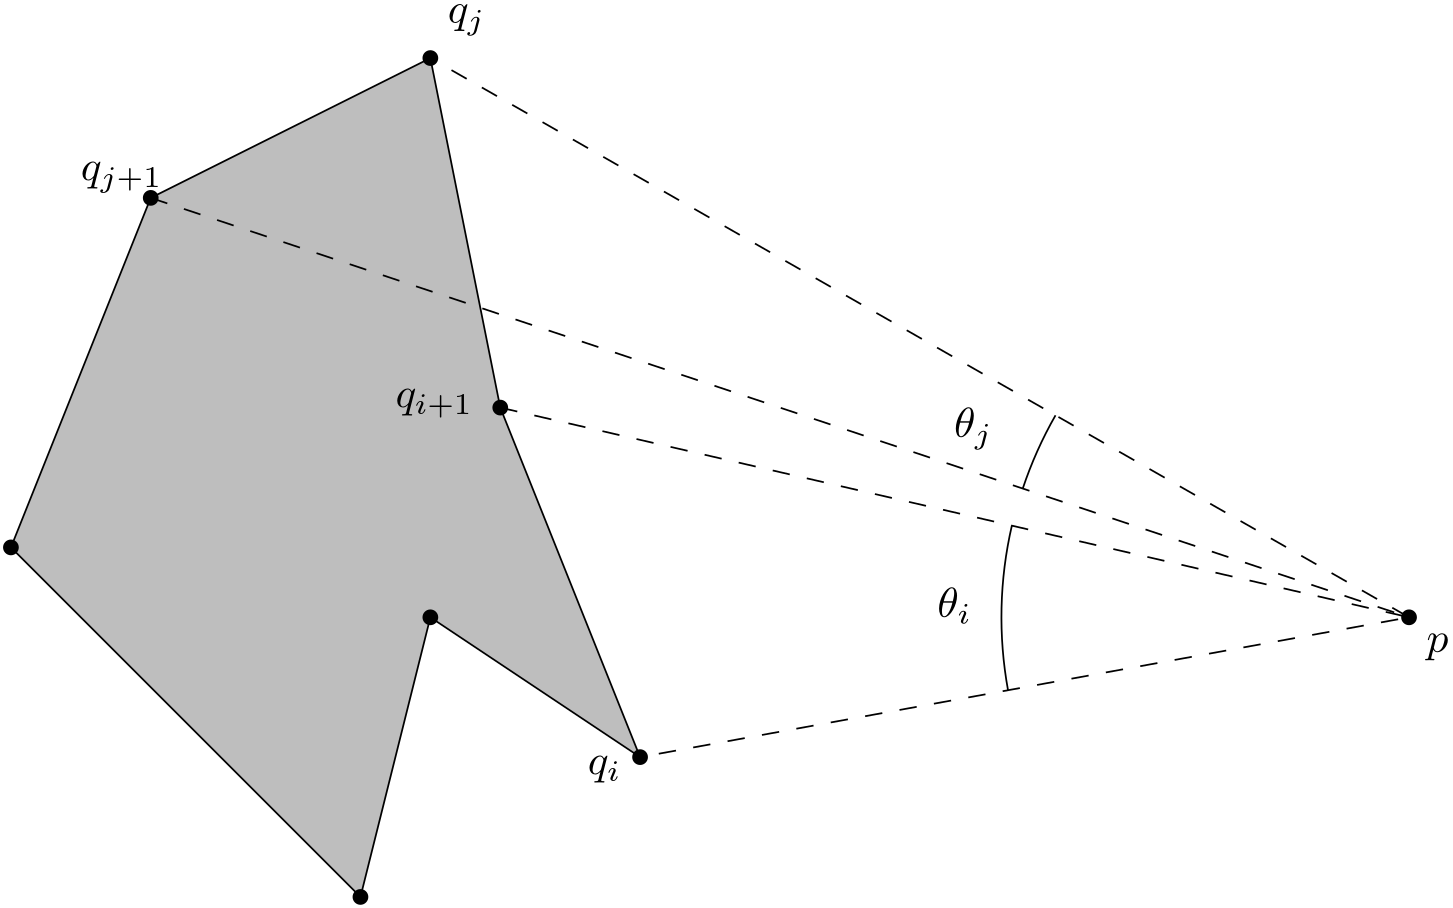
\includegraphics[width=0.8\textwidth]{shapes/point-in-polygon-theta.png}
\برچسب{شکل:چندضلعی-و-زوایا}
\شرح{نمایشِ پارامترهای استفاده شده در الگوریتم}
\پایان{شکل}

حالا می‌دانیم که مسئلهٔ قرارگیریِ نقطه در چندضلعی به مسئلهٔ قولی
\زیرنویس{\lr{promise}}
 به شکلِ زیر تبدیل می‌شود.

\begin{equation}
    \abs{\sum \theta_i s_i} = \begin{cases}
    2\pi & \text{نقطه داخلِ چندضلعی‌ست} \\
    0 & \text{نقطه بیرونِ چندضلعی‌ست}
    \end{cases}
\end{equation}

که به این شکل با این ایده در مرتبهٔ 
$\Theta(N)$
مسئلهٔ مذکور را حل کرد. البته برخلافِ ایدهٔ قبل، نیاز به محاسبهٔ توابعِ وارون‌مثلثاتی‌ست که این کار، سرعتِ این الگوریتم را در واقعیت نسبت به الگوریتمِ قبلی کاهش می‌دهد و از همین‌رو به این ترتیب استفاده نمی‌شود. اما تصحیحاتی بر این الگوریتم وجود دارد که با استفاده از تقریب‌هایی دقت را کاهش می‌دهد اما امکانِ محاسبهٔ سریع را می‌دهد.\مرجع{hormann} 

% TODO that paper in references that is a survay on PIP
